\chapter{Additional results} \label{appendix}

\section{Ground truth engagement measurement} \label{ap:GT}

\begin{figure}[h!]
    \centering
    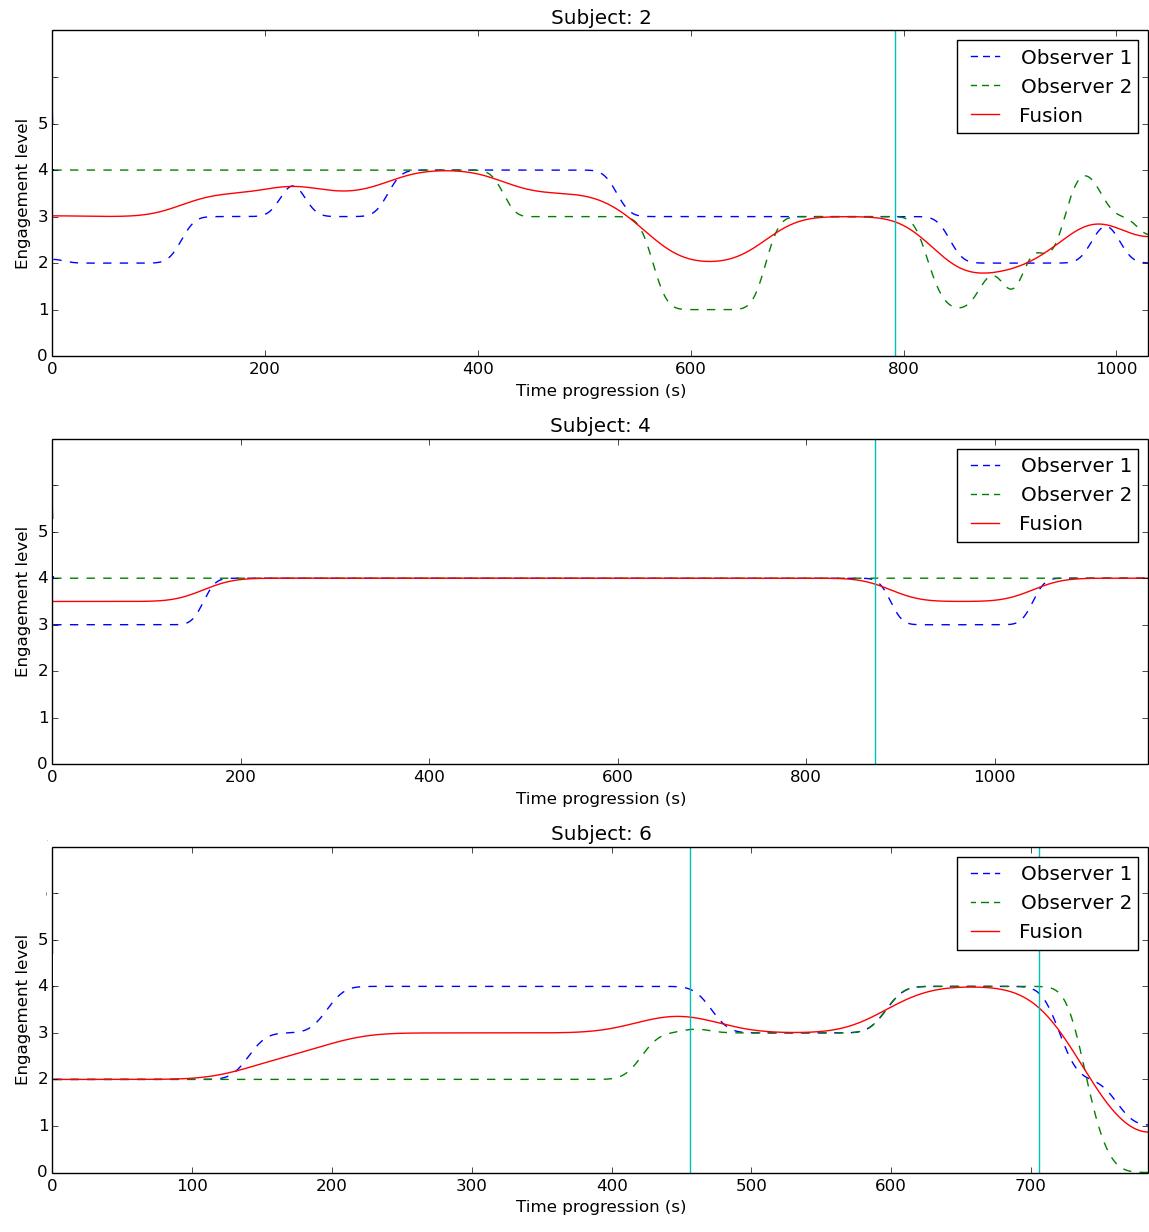
\includegraphics[width=0.6\textwidth]{figures/GT1.png}
    \label{fig:GT1}
\end{figure}
\newpage
\begin{figure}[h!]
    \centering
    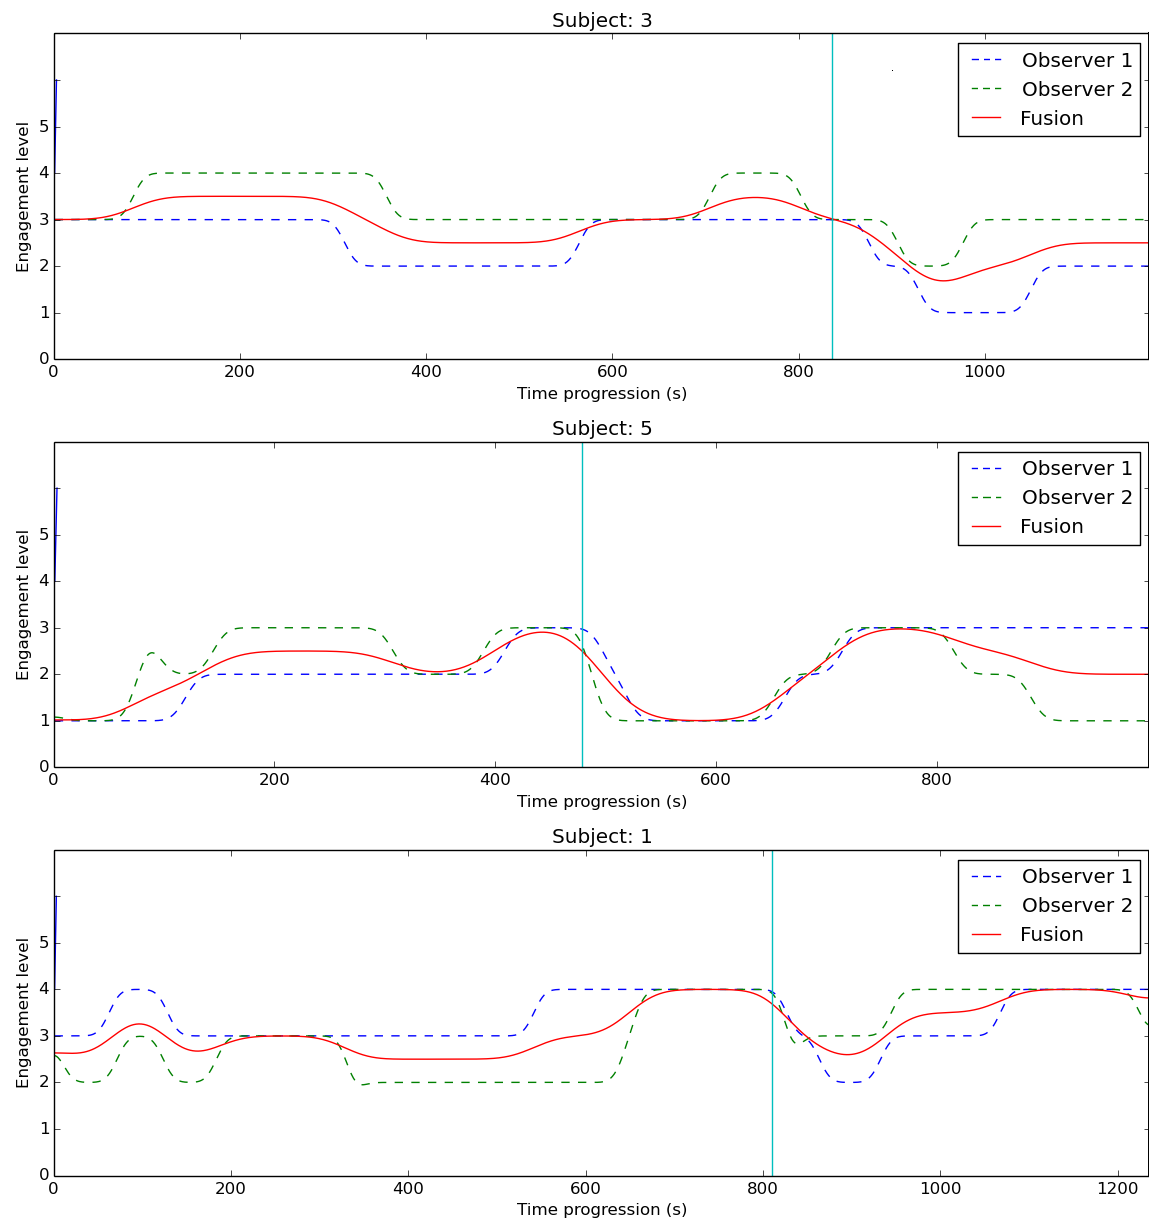
\includegraphics[width=0.6\textwidth]{figures/GT2.png}
    \label{fig:GT2}
    \caption{The 6 Ground Truth acquired during the experiments. The vertical lines indicate the switch to the story telling activity}\label{fig:GTTotal}
\end{figure}

	
\lstinputlisting[basicstyle=\ttfamily\scriptsize,frame=tb,caption=Ground Truth sanity and reliability test,label=zebra]{/home/ferran/Desktop/thesis/R_stuff/GToutput.txt}

\begin{equation} \label{eq:cronbach}
\alpha = {K \over K-1 } \left(1 - {\sum_{i=1}^K \sigma^2_{Y_i}\over \sigma^2_X}\right)
\end{equation}   
where $ \sigma^2_X $ is the variance of the observed total test scores, and $ \sigma^2_{Y_i} $ the variance of component i for the current sample of persons.

\begin{equation}\label{eq:chi}
 \chi^2 = \sum_{i=1}^{n} \frac{(O_i - E_i)^2}{E_i}  
\end{equation}

where $ O_i $ is the number of observations of type \textit{i}, \textit{N} the total number of observations and $ E_i $ the expected (theoretical) frequency of type \textit{i}.

\section{Movement and proximity across the two activities} \label{ap:across}
\lstinputlisting[basicstyle=\ttfamily\scriptsize, float=h,frame=tb,caption= Movement and proximity across activities using T-test,label=zebra]{/home/ferran/Desktop/thesis/R_stuff/acrossOut.txt}
\lstinputlisting[basicstyle=\ttfamily\scriptsize,float=h,frame=tb,caption= One-way repeated measures ANOVA test for proximity,label=zebra]{/home/ferran/Desktop/thesis/R_stuff/repeated1.txt}
\lstinputlisting[basicstyle=\ttfamily\scriptsize,float=h,frame=tb,caption= One-way repeated measures ANOVA test for movement,label=zebra]{/home/ferran/Desktop/thesis/R_stuff/repeated2.txt}


\lstinputlisting[basicstyle=\ttfamily\scriptsize,float=h,frame=tb,caption= Pearson's Chi-squared test result and residual measurements
,label=zebra]{/home/ferran/Desktop/thesis/R_stuff/chi.txt}

%\lstinputlisting[basicstyle=\ttfamily\scriptsize,float=h,frame=tb,caption=
%,label=zebra]{/home/ferran/Desktop/thesis/R_stuff/anovas.txt}

